%% Slides for ".NET Programming" by Chunyu Wang <chunyu@hit.edu.cn> %%

\section{GDI+}

\begin{frame}
\frametitle{GDI+}
\begin{block}{\textit{GDI+ (Graphical Device Interface Plus)}}
  \CJKindent Windows 图形设计界面 (GDI) 的高级实现,可用于创建图形、绘制文本以
  及将图形图像作为对象操作,可以在 Windows 窗体和控件上呈现图形图像。
\end{block}

\begin{itemize}
\item 目前是在 Windows 窗体应用程序中以编程方式呈现图形的唯一方法
\item 虽然无法在 Web 窗体直接使用,但可通过 Web 服务器Image控件显示
\item 所在名字空间

\begin{itemize}
\item System.Drawing 
\item System.Drawing.Drawing2D
\item System.Drawing.Imaging
\item System.Drawing.Text
\item System.Drawing.Printing
\end{itemize}
\end{itemize}
\end{frame}

\begin{frame}[fragile]
\frametitle{Graphics 对象}
\begin{itemize}
\item GDI+ 绘图表面,用来绘制线条、形状、文本或操作图像
\item 获取 Graphics 对象的方法
\begin{itemize}
\item Paint 事件的参数
\begin{lstlisting}[escapeinside=<>]
public void Form1_Paint(object s, PaintEventArgs e) 
{  Graphics g = e.Graphics; <\ldots>  }
protected override void OnPaint(PaintEventArgs e)
{  base.OnPaint(e); <\ldots> }
\end{lstlisting}
\item 控件的 CreateGraphics() 方法
\begin{lstlisting}
   Graphics g = this.CreateGraphics();
\end{lstlisting}
\item 从 Image 对象创建
\begin{lstlisting}[escapeinside=<>]
Bitmap myBitmap = new Bitmap(<imgFileName>);
Graphics g = Graphics.FromImage(myBitmap);
\end{lstlisting}
\end{itemize}
\end{itemize}
\end{frame}


\begin{frame}[fragile]
\frametitle{Graphics 对象}
\begin{itemize}
\item 绘制线条、形状
\begin{lstlisting}[escapeinside=<>]
g.DrawLine(<\ldots>);      g.FillPie(<\ldots>);
g.DrawCurve(<\ldots>);     g.FillRectangle(<\ldots>);
g.DrawPath(<\ldots>);      g.FillPolygon(<\ldots>);
g.DrawPie(<\ldots>);       g.FillRegion(<\ldots>);
\end{lstlisting}
\item 文本
\begin{lstlisting}
g.DrawString(string s, Font f, Brush b, PointF p);
\end{lstlisting}
\item 图像
\begin{lstlisting}[escapeinside=<>]
g.DrawImage(<\ldots>);     g.DrawIcon(<\ldots>);
\end{lstlisting}
\item 变换
\begin{lstlisting}
g.RotateTransform(<\ldots>); g.ScaleTransform(<\ldots>);
\end{lstlisting}
\end{itemize}
\end{frame}

\begin{frame}[fragile]
\frametitle{Pen 和 Brush}
\begin{itemize}
\item Pen 绘制线条
\begin{lstlisting}
  Pen p       = new Pen(Color.Blue, 5);
  p.DashStyle = DashStyle.Dot;
  p.EndCap    = LineCap.ArrowAnchor;
\end{lstlisting}
\item Brush 填充图形
\begin{itemize}
\item SolidBrush 使用纯色绘制
\item HatchBrush 使用预设的图案绘制
\item TextureBrush 使用纹理(如图像)绘制
\item LinearGradientBrush 使用渐变色进行绘制
\item PathGradientBrush 自定义的路径和颜色渐变绘制
\end{itemize}
\begin{lstlisting}
  HatchBrush b = new HatchBrush( HatchStyle.Horizontal,
              Color.Red, Color.FromArgb(128, 255, 255));
  g.FillEllipse(b, 0, 0, 100, 60);
\end{lstlisting}
\end{itemize}
\end{frame}

\begin{frame}[fragile]
\frametitle{Color 对象}
\begin{itemize}
\item 预定义颜色
\begin{lstlisting}
Color color = Color.Red;
\end{lstlisting}
\item 系统颜色
\begin{lstlisting}
Color color = SystemColors.ControlLight;
\end{lstlisting}
\item 自定义颜色
\begin{lstlisting}[escapeinside=<>]
Color color1 = Color.FromArgb(255, 0, 0);
Color color2 = Color.FromArgb(128, 255, 0, 0); //<半透明>
\end{lstlisting}
\end{itemize}
\end{frame}

\begin{frame}[fragile]
\frametitle{GraphicsPath 类}
\begin{lstlisting}
  GraphicsPath gp = new GraphicsPath();
  Point p1 = new Point(50, 100);
  Point p2 = new Point(25, 75);
  Point p3 = new Point(50, 50);
  Point p4 = new Point(75, 50);
  gp.AddBezier(p1,p2,p3,p4);
  g.DrawPath(Pens.Red, gp);
\end{lstlisting}
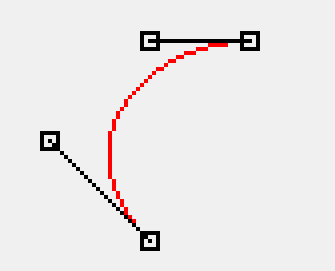
\includegraphics[width=6cm]{gdi-bezier}
\end{frame}

\begin{frame}[fragile]
\frametitle{Range 类}
\begin{lstlisting}
GraphicsPath c1 = new GraphicsPath();
c1.AddEllipse(0, 0, 100, 100);
GraphicsPath c2 = new GraphicsPath();
c2.AddEllipse(60, 0, 100, 100);

Region r1 = new Region(c1);
Region r2 = new Region(c2);
g.FillRegion(Brushes.Red, r1);
g.FillRegion(Brushes.Blue, r2);

r1.Intersect(r2);
g.FillRegion(Brushes.Yellow, r1);
\end{lstlisting}
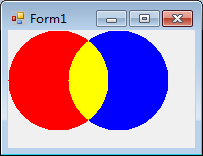
\includegraphics[width=4cm]{gdi-range}
\end{frame}


\begin{frame}[fragile]
\frametitle{图像质量}
\begin{lstlisting}
g.DrawEllipse(new Pen(Color.Red, 6), 10, 10, 20, 20);

g.SmoothingMode = SmoothingMode.AntiAlias;
g.DrawEllipse(new Pen(Color.Blue, 6), 10, 30, 20, 20);
\end{lstlisting}
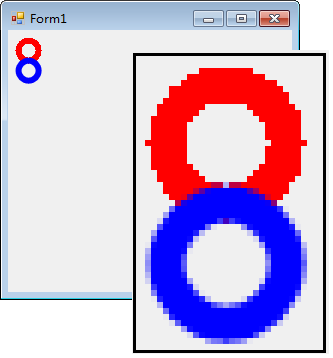
\includegraphics[width=6cm]{gdi-antialias}
\end{frame}

\begin{frame}[fragile]
\frametitle{绘制图形(Image)文件}
\begin{lstlisting}[escapeinside=<>]
Image canvas = new Bitmap(100, 100);
Graphics g = Graphics.FromImage(canvas);
g.Clear(Color.FromArgb(0, 0, 0, 0)); // <透明背景>
g.FillEllipse(Brushes.Red, 6, 60, 60, 60);
g.DrawBezier(new Pen(Color.Blue, 2),
                        0, 0, 80, 30, 20, 70, 100, 100);
canvas.Save(@"d:\dotnet\gdi-image.png", ImageFormat.Png);
\end{lstlisting}

\includegraphics[width=3cm]{gdi-image}
\end{frame}

% \section{其他类库}


% \begin{frame}
% \frametitle{类库纵览}

% \end{frame}

   % 1  Core Types
   % 2  Text
   % 3  Collections
   % 4  Streams and I/O
   % 5  Networking
   % 6  Threading
   % 7  Security
   % 8  Reflection and Metadata
   % 9  Assemblies
   % 10 Serialization
   % 11 Remoting
   % 12 Web Services
   % 13 Data Access
   % 14 XML
   % 15 Graphics
   % 16 Rich Client Applications
   % 17 Web-Based Applications
   % 18 Globalization
   % 19 Configuration
   % 20 Advanced Component Services
   % 21 Diagnostics and Debugging
   % 22 Interoperating with Unmanaged Code
   % 23 Compiler and Tool Support
   % 24 Runtime Facilities
   % 25 Native OS Facilities
   % 26 Undocumented Types


% Local Variables:
% mode: LaTeX
% TeX-master: "part-04.tex"
% TeX-header-end: "% End-of-Header$"
% TeX-trailer-start: "% Start-of-Trailer$"
% coding: utf-8
% End:
